\documentclass{article}
\usepackage[utf8]{inputenc}
\title{video 4: correlation does not usually imply causation (causal inference)}
\author{wbg231 }
\date{December 2022}
\newcommand{\R}{$\mathbb{R}$}
\newcommand{\B}{$\beta$}
\newcommand{\A}{$\alpha$}
\newcommand{\D}{\Delta}

\newcommand{\avector}[2]{(#1_2,\ldots,#1_{#2})}
\newcommand{\makedef}[2]{$\textbf{#1}$:#2 }
\usepackage{tikz,graphicx,hyperref,amsmath,amsfonts,amscd,amssymb,bm,cite,epsfig,epsf,url}

\begin{document}

\maketitle

\section{introduction}
\begin{itemize}
\item \href{https://www.youtube.com/watch?v=dVAGPmiF3E0}{video link}
\item correlation does not imply causation in general, so today we are going to look at casual inference 
\item the issue is confounding variables which can induce correlation between variables that may not otherwise be related. 
\section{working example}
\item for now think we are working with temperature in Spain and unemployment 
\item in the data we see that there is a negative correlation between temperature and unemployment, but is this casual? no likely not
\subsection{ casual inference}
\item key question: when does a treatment t cause a certain outcome
\item in this case does a certain temperature (treatment) cause a certain level unemployment (outcome)
\item potential outcome $\Tilde{po}_{t}$
\item in general we just observe out potential outcome $y=\Tilde{po}_{t}$ when $\Tilde{t}=t$ this is what actually happened 
\item we only see the level of unemployment for the temperature that actually happens 
\item but we are still interested in what would have happened if there was another temperature, think of these as counterfactual
\subsection{potential outcome }
\item suppose we see one observed outcome but all treatments lead to the same potential outcome 
\item like this 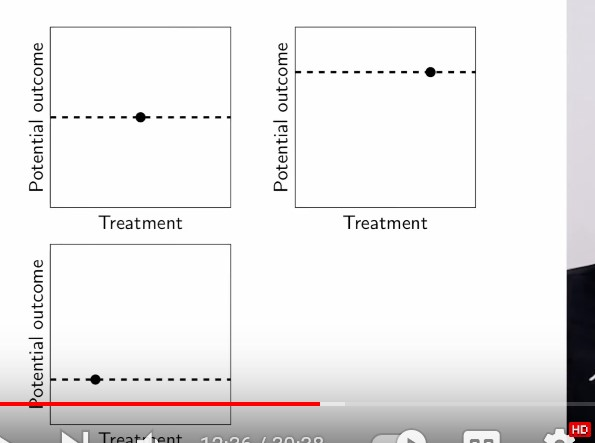
\includegraphics[width=5cm]{notes/week_2/potential_outcome.jpg}
\item the issue is we only observe one value, so it is hard to reason about the counterfactual. 
\item but we only work with observed data like this 
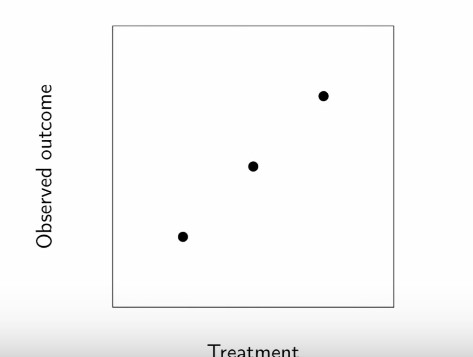
\includegraphics[width=5cm]{notes/week_2/observed_data.jpg}
\item this seems to show some correlating 
\section{linear casual effect}
\item here we are looking for a linear causal effect that is we assume there exists come constant $\beta \in \mathbb{R}$ such that $E[\Tilde{po}_{t}]=\beta t$
\item that is the mean of the potential outcome is proportional to value of the treatment
\item if we increase the temperature by 1 degree the unemployment goes down by $\beta$ percent
\item can we estimate this from data
\section{idea}
\item we want to use covariance between outcome y and treatment y 
\item we can do this but we must assume that the potential outcome $\Tilde{po}_{t}$ and treatment (t) are independent for all values of t 
\item naturally this does not mean $y\perp t$ that is the observed outcome is independent from treatment
\item instead it just means the selection of the treatment is independent from the outcome 
\subsection{iterated expectations}
\item suppose that $E[t]=0$ and $e[t^2]=var(t)=1$
\item so here we can use iterated expectations to say $cov(y,t)=E[yt]-e[y]e[t]=E[yt]=E[\mu_{yt|t}(t)]$
\item note that $\mu_{yt|t}(t)=\int_{y\in Y}ytf_{y|t}(y|t)dy=\int_{y\in Y}tyf_{\Tilde{po}_{t}}(y|t)dy$ then as $\Tilde{po}_{t}\perp t$ we have $\mu_{yt|t}(t)=\int_{y\in Y}ytf_{y|t}(y|t)dy=\int_{y\in Y}tyf_{\Tilde{po}_{t}}(y|t)dy=t\int_{y\in Y}yf_{\Tilde{po}_{t}}(y)dy=tE[\Tilde{po}(t)]$ then finally by our linear casual effect assumption we can write $\mu_{yt|t}(t)=tE[\Tilde{po}(t)]=t\beta t=\beta t^2$
\item then we can write $cov(y,t)=E[yt]-e[y]e[t]=E[yt]=E[\mu_{yt|t}(t)]=E[\beta t^2]=\beta E[t^2]=\beta $ so thus we see that in this case the covariance between the treatment and outcome capture the linear casual effect as long as the Independence between treatment and potential outcome assumption is met 
\section{why do we need impertinence}
\item because if we do not have Independence between treatment and potential outcome it is possible for confounders to cause a spurious correlations 
\item however in practice it is very hard to randomize 
\section{Spain example}
\item if we account for tourism in the Spain example, then we can isolate the correlation between unemployment and temperature.
\item that is because tourism is a confound
\section{example}
\item suppose we want gunny pigs to gain weight and want to know if a supplement helps with this 
\item first we give them supplements then food and notice that those individuals that eat more supplement gain weight 
\item then the next week we repeater the experiment but give them the supplement after the  food and observe a negative correlation between supplement and weight gain.
\item so finally we randomize the treatment ie the amount of supplement each individual gets and we see that there is zero correlation between weight change and supplement 
\item this tells us that there is a confound in this relationship. here the confound is the food intake of an individual
\item so we can say there is for sure a relationship between weight gain and food intake. 
\item if we give the gunny pigs supplement before food then we see that individuals that eat more supplement also eat more food
\item if we give the gunny pigs supplement after food then we see that individuals that eat more supplement also eat less food because they are already full leaning to a spurious negative relationship
\item when we randomize supplement level food intake and the supplement level are no longer related and this controls for that confound. allowing us to see there is no linear relationship between weight gain and supplement 
\section{unobserved confounder}
\item potential outcome $\Tilde{po}_{t,c}$ depends both on treatment t and confounder c 
\item observed data $y=\Tilde{po}_{t,c}$ where $\Tilde{t}=t,\Tilde{c}=c$
\item suppose there is a linear relationship such that $\beta \gamma \in \mathbb{R}$ we have $E[\Tilde{po_{t,c}}]=\beta t+ \gamma c$
\item can we still estimate the covariance between t and y ignoring c? like for instance if we don't know about c 
\item assume that t and c are standardised and that there are no additional confounders that is $\Tilde{po}_{t,c}\perp (t,c)$
\item so we can say $cov(y,t)=E[yt]-e[y]e[t]=E[yt]=E[\mu_{yt|t,c}(t,c)]$
\item note that $\mu_{yt|t,c}(t,c)=\int_{y\in Y}ytf_{y|t,c}(y|t,c)dy$ since t and c are held constant we can write this as $\int_{y\in Y}tyf_{\Tilde{po}_{t,c}}(y|t,c)dy$ now with Independence and no additional confounders we can write this $\int_{y\in Y}tyf_{\Tilde{po}_{t,c}}(y)dy=tE[\Tilde{po}_{t,c}]=t(\beta t+\gamma c)=\beta t^2+\gamma tc $
$cov(y,t)=E[yt]-e[y]e[t]=E[yt]=E[\mu_{yt|t,c}(t,c)]=E[\beta t^2+\gamma tc]=\beta +\gamma \rho_{t,c}$ so we the real relationship $\beta $ plus some distorting factor $\gamma\rho_{t,c}$ which is effected by the relationship between the treatment and confounder t,c $\rho_{t,c}$
\item if there is no relationship between t,c that is they are linearly independent or uncorrelated that $cov(y,t)=E[yt]-e[y]e[t]=E[yt]=E[\mu_{yt|t,c}(t,c)]=E[\beta t^2+\gamma tc]=\beta +\gamma \rho_{t,c}=\beta$ which means that we would view the correct relationship we want to see 

\end{itemize}
\end{document}
